
% Background Chapter: Expanded and Enhanced
\subsection*{1. Origins of Threat Modeling}
Threat modeling has evolved from a niche security practice to a central pillar of modern cybersecurity strategy. In the earliest days of computing, security focused on defending the network perimeter—firewalls, access controls, and antivirus software were the primary tools. As Bruce Schneier observed\cite{schneier1999}, this reactive approach left many systems exposed to sophisticated attacks exploiting design, implementation, and business logic flaws. The rise of the internet and interconnected systems in the 1980s and 1990s fundamentally changed the threat landscape, making perimeter defenses alone insufficient.

\subsection*{2. Early Security Practices and Limitations}
During the 1980s and 1990s, organizations began to recognize the limitations of traditional security models. Attackers found new ways to bypass controls, and insider threats became more prominent. The need for a proactive, systematic approach to risk management led to the development of structured threat modeling methodologies. Security professionals started to look beyond technology, considering organizational context, regulatory requirements, and adversary tactics.

\subsection*{3. The Emergence of Structured Frameworks}
The late 1990s marked a turning point with the introduction of the STRIDE framework by Microsoft\cite{shostack2014}. STRIDE provided a repeatable process for identifying and categorizing threats during the software design phase, enabling teams to address security concerns before deployment. Around the same time, Carnegie Mellon University developed OCTAVE\cite{nist800154}, focusing on organizational risk and asset-based analysis. The PASTA methodology\cite{uceda2015} emphasized attacker simulation and business impact, while community-driven resources like OWASP\cite{owasp} promoted practical, actionable guidance for developers and security teams.

\subsection*{4. Key Milestones in Threat Modeling}
The evolution of threat modeling is marked by several key milestones:
\begin{itemize}
	\item \textbf{1999: STRIDE} — Microsoft introduces STRIDE, integrating threat modeling into the Secure Development Lifecycle (SDL) and establishing a foundation for modern security engineering\cite{shostack2014}.
	\item \textbf{2001: OCTAVE} — Carnegie Mellon University develops OCTAVE, focusing on organizational risk and asset-based analysis, and promoting a holistic view of security\cite{nist800154}.
	\item \textbf{2012: PASTA} — The Process for Attack Simulation and Threat Analysis (PASTA) is published, emphasizing attacker perspective, business impact, and the integration of technical and business analysis\cite{uceda2015}.
	\item \textbf{2010s: VAST, Trike, and OWASP} — New frameworks emerge to address scalability, risk quantification, agile development, and community-driven best practices\cite{owasp}.
\end{itemize}

\begin{figure}[H]
	\centering
	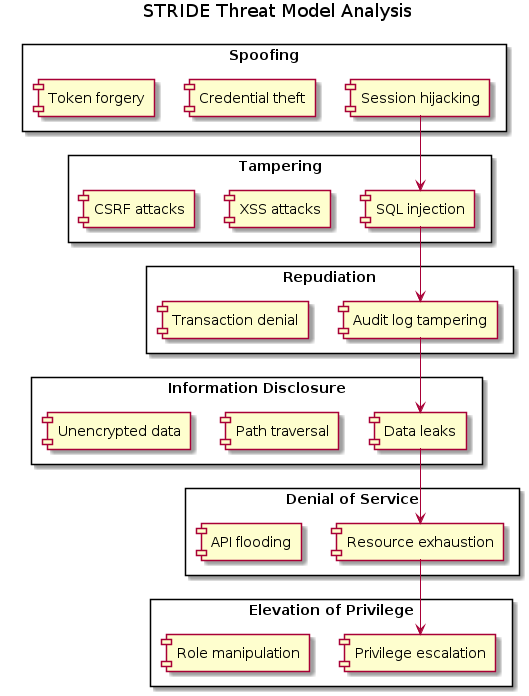
\includegraphics[width=0.8\textwidth]{images/stride-analysis}
	\caption{Timeline of Major Threat Modeling Frameworks}
\end{figure}

\subsection*{5. Modern Threat Modeling: Tools, Standards, and Practice}
Today, threat modeling is a mature discipline supported by a wide range of tools, methodologies, and community resources. It is recognized as a best practice by standards bodies (NIST SP 800-154\cite{nist800154}, ISO 27001), regulatory frameworks (GDPR, HIPAA), and industry groups (OWASP\cite{owasp}). Modern threat modeling addresses not only technical vulnerabilities but also business logic, supply chain risks, and emerging technologies such as cloud, IoT, and artificial intelligence. The field continues to evolve, with new approaches and tools emerging to meet the challenges of increasingly complex and interconnected systems.

\subsection*{6. Academic and Industry Collaboration}
The history of threat modeling reflects decades of research, real-world experience, and collaboration between industry, academia, and the security community. Leading books such as Shostack’s "Threat Modeling"\cite{shostack2014}, UcedaVélez and Morana’s "Risk Centric Threat Modeling"\cite{uceda2015}, and Schneier’s "Secrets and Lies"\cite{schneier1999} provide foundational knowledge. Standards like NIST SP 800-154\cite{nist800154} and resources from OWASP\cite{owasp} ensure that best practices are accessible and actionable for organizations of all sizes.

\subsection*{7. Summary and Looking Forward}
Understanding the evolution of threat modeling helps organizations appreciate its value and apply its principles to build more secure and resilient systems. As threats continue to evolve, so too must the methodologies and tools used to defend against them. The next chapters will explore the technical definitions, frameworks, and practical applications that underpin modern threat modeling.
